\chapter{Studio del funzionamento}
\label{cha:analysis}

\section{Il sistema dal punto di vista dell'utente}
\label{sec:ux}

Il sistema FAAC SLH a 2 canali presenta due componenti:
\begin{itemize}
  \item Il ricevitore: una PCB con due pulsanti per gestire tutte le funzioni di memorizzazione dei radiocomandi e 4 dipswitch per gestire la modalità di operazione.
  \item I radiocomandi: semplici trasmettitori a due pulsanti e un led memorizzabili nel ricevitore.
\end{itemize}
Il ricevitore offre una semplice procedura per memorizzare e sincornizzare i radiocomandi, procedura dopo la quale il radiocomando potrà essere utilizzato per il suo scopo. Il sistema FAAC SLH è progettato per essere tollerante: nel caso in cui alcuni segnali del trasmettitore non raggiungano la destinazione, il ricevitore si risincronizzerà (entro alcuni limiti) automaticamente.\\
Inoltre i trasmettitori offrono due funzionalità:
\begin{itemize}
  \item TX coding: un trasmettitore può trasmettere la sua chiave di sistema ad un altro trasmettitore che cambierà la propria chiave di distema in quella appena ricevuta effettivamente clonando il primo.
  \item Master/Slave: di fabbrica un trasmettitore è “master”, ciò vuol dire che può trasmettere la sua chiave di sistema. Tramite la pressione dei pulsanti in una determinata sequenza un master può essere trasformato in “slave”, quest’ultimo viene permanentemente privato della capacità di trasmettere la sua chiave di sistema ma non di assumerne altre.
\end{itemize}
Varie revisioni dei manuali  \cite{man1,man2} dei radiocomandi riportano più o meno informazioni sulle funzionalità dei prodotti.

\section{La trasmissione}
\label{sec:transmission}

\subsection{Segnale ed interpretazione}
\label{sub:signal}

Primo passo nello studio del sistema FAAC SLH è intercettare un segnale per capirne la struttura e la funzione. A questo scopo il Flipper Zero si rivela estremamente utile vista la funzionalità di ricezione di segnali SubGHz già implementata in dettaglio. Utilizzando la funzione “Read RAW” del Flipper Zero possiamo ottenere una lettura non processata del segnale. Questa lettura viene esportata dal Flipper Zero in un file (estensione sub) che riporta le seguenti informazioni:
\begin{itemize}
  \item Filetype: il tipo e contenuto del file
  \item Version: un informazione interna riguardo la versione del’implementazione
  \item Frequenza: la frequenza di ricezione del segnale
  \item Preset: impostazioni di ricezione come modulazione e ampiezza d’onda
  \item Protocollo: il protocollo se risconosciuto (RAW se in modalità raw)
  \item Data: la trasmissione effettivamente ricevuta
\end{itemize}
Per la lettura di un segnale FAAC SLH si usano queste impostazioni:
\begin{itemize}
  \item Frequenza: 433.92MHz
  \item Modulazione: AM270 (rappresenta una modulazione On/Off Keying con ampiezza d’onda di 270kHz)
\end{itemize}
Una lettura così effettuata genererà un file il cui campo “Data” è popolato con una serie di numeri alternativamente positivi e negativi che rappresentano rispettivamente segnale alto e silenzio di lunghezza specificata dal valore assoluto del numero (valore 1 = 1 microsecondo). Osservando queste informazioni si possono estrarre numerose informazioni:
\begin{itemize}
  \item Il segnale del trasmettitore sembra iniziare con un segnale di circa 150ms seguito da un silenzio lungo altrettanto
  \item Una coppia di segnale di 0.3ms e silenzio di 0.3ms viene inviata 8 volte, questa sequenza sembra essere un segnale introduttivo che annuncia l’arrivo della sequenza di dati
  \item una coppia di un segnale lungo 1.1ms e un silenzio lungo altrettanto è inviata, questa sequenza sembra essere un preambolo alla sequenza di dati che rappresenta il payload principale
  \item 64 coppie di segnale e silenzio sono inviate, questa sequenza sembra essere il payload della trasmissione. Queste coppie si configurano in solo due possibili modi:
    \begin{itemize}
      \item Segnale lungo (0.6ms) seguito da silenzio corto (0.3ms)
      \item Segnale corto (0.3ms) seguito da silenzio lungo (0.6ms)
    \end{itemize}
  \item A questo punto il segnale si ripete a partire dal preambolo fino al rilascio del pulsante del trasmettitore
\end{itemize}
Appare quindi chiaro che le 64 coppie segnale-silenzio rappresentino un payload di 64bit in cui ogni coppia rappresenta un bit 1 o 0.\\
Il codice sorgente del firmware del Flipper Zero (sia originale che Unleashed) rivela che:
\begin{itemize}
  \item Segnale corto seguito da silenzio lungo corrisponde al bit 0
  \item Segnale lungo seguito da silenzio corto corrisponde al bit 1
\end{itemize}
A questo punto è triviale ottenere il payload a partire da questi dati, una funzione per ciò è già implementata nel Flipper Zero nel file \texttt{lib/subghz/protocols/faac\_slh.c}\cite{firmware}.

\subsection{Struttura del pacchetto dati}
\label{sub:payload}
D’ora in poi con il termine “chiave” si intenderà il pacchetto dati di 64 bit inviato dal trasmettitore.\\
Il trasmettitore FAAC SLH può trasmettere due chiavi differenti:
\begin{itemize}
  \item Chiave normale: inviata alla pressione normale di uno dei pulsanti, è il pacchetto standard inviato quando il radiocomando deve autenticarsi nel ricevitore.
  \item Chiave di programmazione: inviato alla pressione di uno dei pulsanti mentre il trasmettitore è in modalità “Programmazione”, all’interno del codice del firmware “Unleashed” viene soprannominato “Master Remote Prog Key”.
\end{itemize}
Analizziamo prima la chiave normale che, secondo la rappresentazione esadecimale di 64 bit, prenderà questa forma:
\begin{center}
  \texttt{XX XX XX XY ZZ ZZ ZZ ZZ}
\end{center}
I 4 byte più significativi (\texttt{XX XX XX XY}) rappresentano quello che viene soprannominato “code fix”. Questa porzione contiene il numero seriale, detto “serial”, del trasmettitore (\texttt{XX XX XX X}, 28 bit) e il valore del tasto premuto (\texttt{Y}, 4 bit), detto “button”. Chiaramente il serial non varia mai per un trasmettitore mentre il button varia in base al pulsante premuto\footnote{Il code fix può cambiare quando il radiocomando è trasformato in slave ma mai in operazione normale}.\\
4 byte (32 bit) meno significativi (\texttt{ZZ ZZ ZZ ZZ}) rappresentano quello che viene soprannominato “code hop”, ovvero il codice a rotazione in sé. Ovviamente il code hop cambia ad ogni trasmissione.\\
Si potrebbe pensare a questi due elementi come l’username (il code fix) e la password (il code hop) di un tradizionale login form.
Si è rilevato che il ricevitore apparentemente accetti esclusivamente trasmettitori con valore serial entro il range [A0000000--A0FFFFFF] in questa maniera:\\
\begin{itemize}
  \item Si emulano vari radiocomandi FAAC SLH tramite la funzionalità “Add manually” > “Faac SLH 433MHz” sul Flipper Zero (firmware Unleashed necessario)
  \item Si inviano vari segnali con vari differenti valori di “code fix”, count invariato e seed invariato
  \item Si osserva che solo valori di code fix compresi nel range precedentemente menzionati si autenticano correttamente nel ricevitore.
\end{itemize}
Non può essere escluso che altri valori vengano accettati dal ricevitore vista l’implausibilità di testare tutte le combinazioni di 32 bit, tuttavia è ragionevole pensare che sia l’implementazione effettiva interna al ricevitore. Il range sopra menzionato offre 16\^6 possibili code fix.\\
Analizziamo ora la chiave di programmazione che prende questa forma:
\begin{center}
  \texttt{52 0F XX XX XX XX YY 00}
\end{center}
Si può osservare come questa chiave sia contraddistinta dai primi 2 byte più significativi e dal byte meno significativo che rimangono costanti a qualsiasi trasmissione di questo tipo. Si può ipotizzare che sia questo il meccanismo con cui il ricevitore riconosce il tipo di chiave ricevuta.\\
Il contenuto di questa chiave è diviso in \texttt{XX XX XX XX} che rappresenta il valore del seed codificato e \texttt{YY}, valore che viene chiamato mCnt necessario alla decodifica del seed.\\
La chiave è trasferita in modalità Big Endian.

\section{Implementazione del codice a rotazione}
\label{sec:rolling}

\subsection{KeeLoq}
\label{sub:keeloq}

Fonti: \cite{keeloqwiki,keeloqc,algebraic_slide,cryptoeprint,periodic_ciphers}.\\

\begin{wrapfigure}
  {r}{.5\textwidth} %
  \centering
  \def\stackalignment{r}\stackunder{
    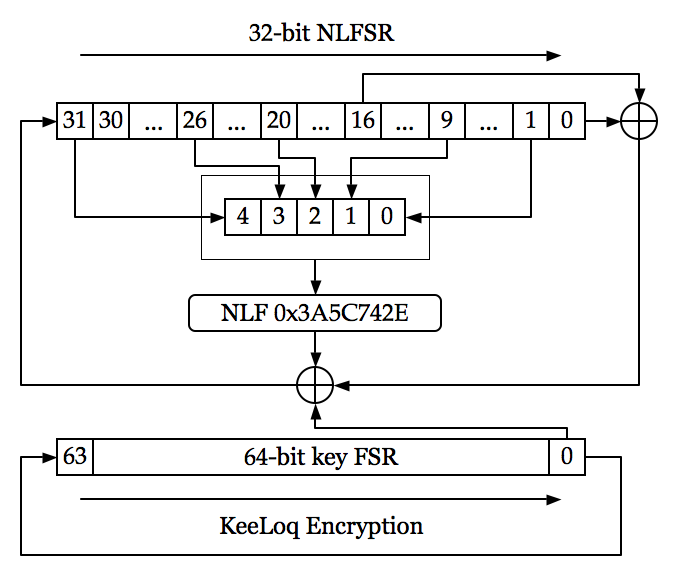
\includegraphics[width=\linewidth]{images/encrypt.png}
  } %
  {\scriptsize \parbox[t]{\linewidth}{ Fonte: \cite{keeloqwiki}} }
  \caption{Fase di encrypt in KeeLoq}
  \label{fig:keeloq_encrypt}
\end{wrapfigure}
Come menzionato precedentemente FAAC SLH sfrutta l’algoritmo KeeLoq per l’implementazione del codice a rotazione. Ai fini di questo studio non è necessaria una conoscenza troppo approfondita di questo algoritmo, difatti si potrebbe semplicemente considerarlo un black box algorithm che prende in input un payload e la chiave ed è in grado di crittografare o decrittografare i dati. Tuttavia risulta utile comprenderne a grandi linee il funzionamento per capire come FAAC SLH lo integra.\\
Keeloq, a partire dagli anni ‘80, gode di ampio utilizzo in sistemi di RKE per veicoli, barriere fisiche e sistemi di allarme.\\
L’algoritmo KeeLoq sfrutta due registri da 32 bit (stato) e 64 bit (chiave) che, rispettivamente, operano come Non-Linear Feedback Shift Register (NLFSR) e registro circolare e, sempre rispettivamente, sono inizializzati con il plaintext e la chiave segreta. Un initialization vector (IV) è utilizzato in certe implementazioni per inizializzare il registro a 32 bit e garantire un cifrario differente per lo stesso messaggio.
Il ciclo principale di crittografia dell’algoritmo è composto di 528 iterazioni per ognuna delle quali il feedback dell’NLFSR dipende da i bit 1, 9, 20, 26 e 31 del registro di stato e da una specifica Non-Linear Feedback Function (NLF) data da: \(NLF(a, b, c, d, e) = d \oplus e \oplus ac \oplus ae \oplus bc \oplus be \oplus cd \oplus de \oplus ade \oplus ace \oplus abd \oplus abc\), funzione rappresentabile dall’esadecimale 0x3A5C742E. L’output di questa funzione viene quindi combinato linearmente (XORed) con i bit 0 e 16 del NLFSR e dal bit 0 del registro chiave nel suo attuale stato. Il risultato di questa serie di operazioni viene reinserito nel NLFSR. Dopo ogni iterazione entrambi i registri scorrono di un bit a destra. Il risultato finale si ottiene dallo stato finale del registro di stato dopo le 528 iterazioni. Il vettore di inizializzazione del registro di stato è tipicamente sottoposto a XOR con i bit meno significativi della chiave sia prima che dopo le iterazioni.\\

\begin{wrapfigure}
  {r}{.5\textwidth} %
  \centering
  \def\stackalignment{r}\stackunder{
    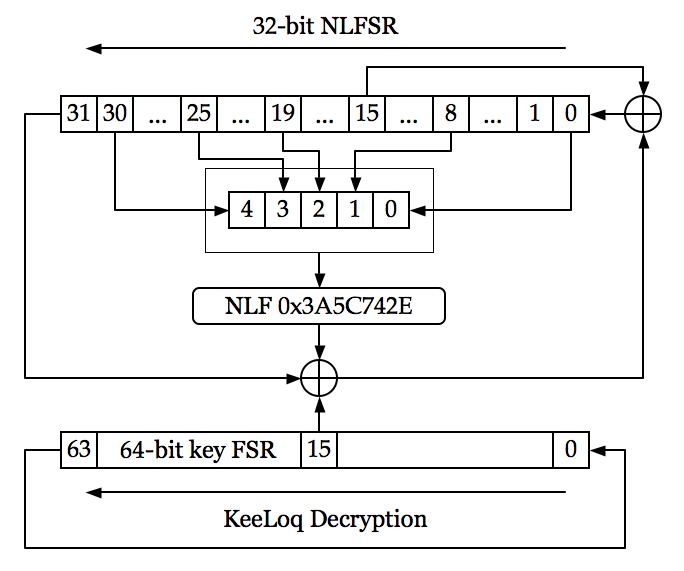
\includegraphics[width=\linewidth]{images/decrypt.png}
  } %
  {\scriptsize \parbox[position]{\linewidth}{ Fonte: \cite{keeloqwiki}} }
  \caption{Fase di decrypt in KeeLoq}
  \label{fig:keeloq_decrypt}
\end{wrapfigure}

Il processo di decrittografia avviene in maniera simile a quello di crittografia con alcune differenze chiave:
\begin{itemize}
  \item Il registro di stato è inizializzato con il testo cifrato
  \item La NLF dipende da un insieme diverso di bit di stato: 0, 8, 19, 25 e 30
  \item L’output della NLF è sottoposto a XOR con bit differenti dello stato (31 e 15) e della chiave (15)
  \item Il registro di stato scorre verso sinistra
\end{itemize}
Seppure la NLF introduca un fattore di non linearità è facile notare la semplicità della struttura e la lunghezza relativamente limitata della chiave a 64 bit. Inoltre vari attacchi criptoanalitici hanno sfruttato l’esistenza di approssimazioni lineari efficienti della NLF ed il fatto che l’utilizzo e l’aggiornamento della chiave dopo 64 round si ripete.

\subsection{KeeLoq in FAAC SLH}
\label{sub:faacslh}

Per comprendere l’implementazione di KeeLoq a rotazione di FAAC SLH osserviamo il procedimento di memorizzazione nel ricevitore, il contenuto della chiave di programmazione e il codice sorgente del firmware Unleashed.\\
Il procedimento per memorizzare il trasmettitore nel ricevitore si compone di queste fasi:
\begin{itemize}
  \item Tramite un pulsante sul ricevitore si imposta quest’ultimo in modalità “Programmazione”
  \item Si invia una chiave di programmazione con il trasmettitore, il ricevitore quindi uscirà dalla modalità programmazione
  \item Si inviano due chiavi normali col trasmettitore e alla seconda ricevuta il ricevitore sarà sincronizzato e aprirà la barriera
\end{itemize}
Ricordiamo il formato della chiave di programmazione:
\begin{center}
  \texttt{52 0F XX XX XX XX YY 00}
\end{center}
in cui \texttt{XX XX XX XX} è il seed codificato e \texttt{YY} è una chiave di decodifica.
La routine della decodifica del seed si compone di un ciclo che itera sul valore del seed codificato YY volte il cui corpo è composto di semplici manipolazioni bitwise del valore in funzione di mCnt. Questo routine sembra un modo di offuscare il valore del seed durante la trasmissione ma risulta, tuttavia, estremamente debole.\\
Il codice responsabile di questo processo nel firmware Unleashed è riportato nell'appendice A.\\
Una volta ottenuto il seed, il ricevitore esce dalla modalità di programmazione e torna in modalità di ascolto normale, si può quindi supporre che il seed venga salvato internamente per inizializzare un counter interno.\\
Le successive due chiavi normali trasmesse, se sequenziali, sincronizzeranno il ricevitore con il trasmettitore.\\
Ricordiamo ora la struttura delle chiavi normali:
\begin{center}
  \texttt{XX XX XX XX YY YY YY YY}
\end{center}
dove \texttt{XX XX XX XX} è detto “code fix” e \texttt{YY YY YY YY} è detto “code hop”.\\
Il code fix è composto a sua volta da numero seriale “serial” e pulsante premuto “btn” ma a livello di funzionalità del ricevitore non è necessario distinguere queste due parti.\\
Il codice del firmware Unleashed offre l’implementazione di KeeLoq in FAAC SLH per la decrittografia del code hop. Ricordiamo che l’algoritmo di KeeLoq crittografa un payload di 32 bit con una chiave di 64 bit. La chiave di 64 bit è ottenuta nella seguente funzione a partire dal seed e dalla cosiddetta “Manufacturer key”, una chiave costante segreta legata a FAAC SLH.\\
É interessante il fatto che per ottenere la chiave da 64 bit la funzione di learning esegua l’intero algoritmo di KeeLoq nella versione di encrypt due volte.\\
Ottenuta la chiave di 64 bit si estrae il valore del counter dal risultato della decrittografia.\\
Il codice di questi vari procedimenti è riportato nell'appendice B.\\
Due note:
\begin{itemize}
  \item Il count è composto di solo 5 cifre esadecimali (5 nibble)
  \item A volte la lettura della chiave di programmazione di un singolo radiocomando effettuata col Flipper Zero riporta un risultato peculiare differente dal normale: se il seed di un radiocomando è XX XX YY YY a volte YY YY XX XX viene letto. Non è chiaro se questo fatto risulti da un errore nell’implementazione del protocollo nel firmware Unleashed o se sia un comportamento anomalo del radiocomando.
\end{itemize}
In base a quanto dedotto dal codice del firmware, il code fix non entra in gioco nel processo di decodifica del valore count, infatti, come sarà spiegato successivamente, il ruolo di questo valore è cruciale nella sincornizzazione di multipli radiocomandi sullo stesso ricevitore.\\
É importante sottolineare come il processo appena descritto avviene nel Flipper Zero durante la lettura dei segnali FAAC SLH e non nel ricevitore originale FAAC SLH: è altamente probabile che internamente il ricevitore segua una logica ben differente quando si tratta di decriptare ed autenticare i segnali ricevuti, tuttavia la logica di KeeLoq rimane valida. Per esempio si potrebbe ipotizzare che il ricevitore decripti il segnale ricevuto dal radiocomando e verifichi il valore del counter, oppure che il ricevitore stesso calcoli il code hop previsto e verifichi che quello ricevuto corrisponda.\\


